%%%%%%%%%%%%

%%%%%%%%%%%%
% Basic setup

\documentclass[letterpaper,11pt]{article}
\usepackage[dvipsnames]{xcolor}
\usepackage{fullpage}
\usepackage{etaremune}
\usepackage{setspace}
\usepackage{textcomp}
\usepackage{fancyhdr}
\usepackage{fontawesome}
\usepackage{enumitem}
\usepackage{ifthen}
\usepackage{ifpdf}
\usepackage{catchfile}
\usepackage{tikz}
\usepackage{geometry}
\usepackage{lastpage}
\usepackage{eso-pic}
\usepackage{transparent}
\usepackage{eso-pic}
\usepackage{calc}
\usepackage{microtype}

\usepackage{pgfornament}
\usepackage{tikz}
\usetikzlibrary{calc}

%%%%%%%%%%%%
% Last updated

\AddToShipoutPictureBG*{%
  \AtPageUpperLeft{%
    \put(\LenToUnit{\paperwidth-\oddsidemargin-1.075in},\LenToUnit{-9.5mm}){%
      \makebox[0pt][r]{\footnotesize\textcolor{gray!80}{\textit{Last updated: \today}}}%
    }%
  }%
}

%%%%%%%%%%%%
% Subtle \mid separator

\newcommand{\lightsep}{\textcolor{gray!80}{$\mid$}}

%%%%%%%%%%%%
% Link colour

\newcommand\myshade{85}
\colorlet{linkcolor}{Maroon}

%%%%%%%%%%%%
% Spacing

\setstretch{1.155}

%%%%%%%%%%%%
% Logos

\newcommand{\arxivlogo}{
\includegraphics[height=1em]{figures/arxiv-logo.pdf}}
\newcommand{\inspirelogo}{
\includegraphics[height=1em]{figures/inspire-logo.pdf}}
\newcommand{\adslogo}{
\includegraphics[height=1em]{figures/ads-logo.pdf}}
\newcommand{\scholarlogo}{
\includegraphics[height=1em]{figures/gscholar-logo.pdf}}


%%%%%%%%%%%%
% Background pic

\newcommand\BackgroundPic{%
\put(-2mm,1.\paperheight / 2.){
\parbox[b][\paperheight]{\paperwidth}{%
\vfill
%\transparent{0.1}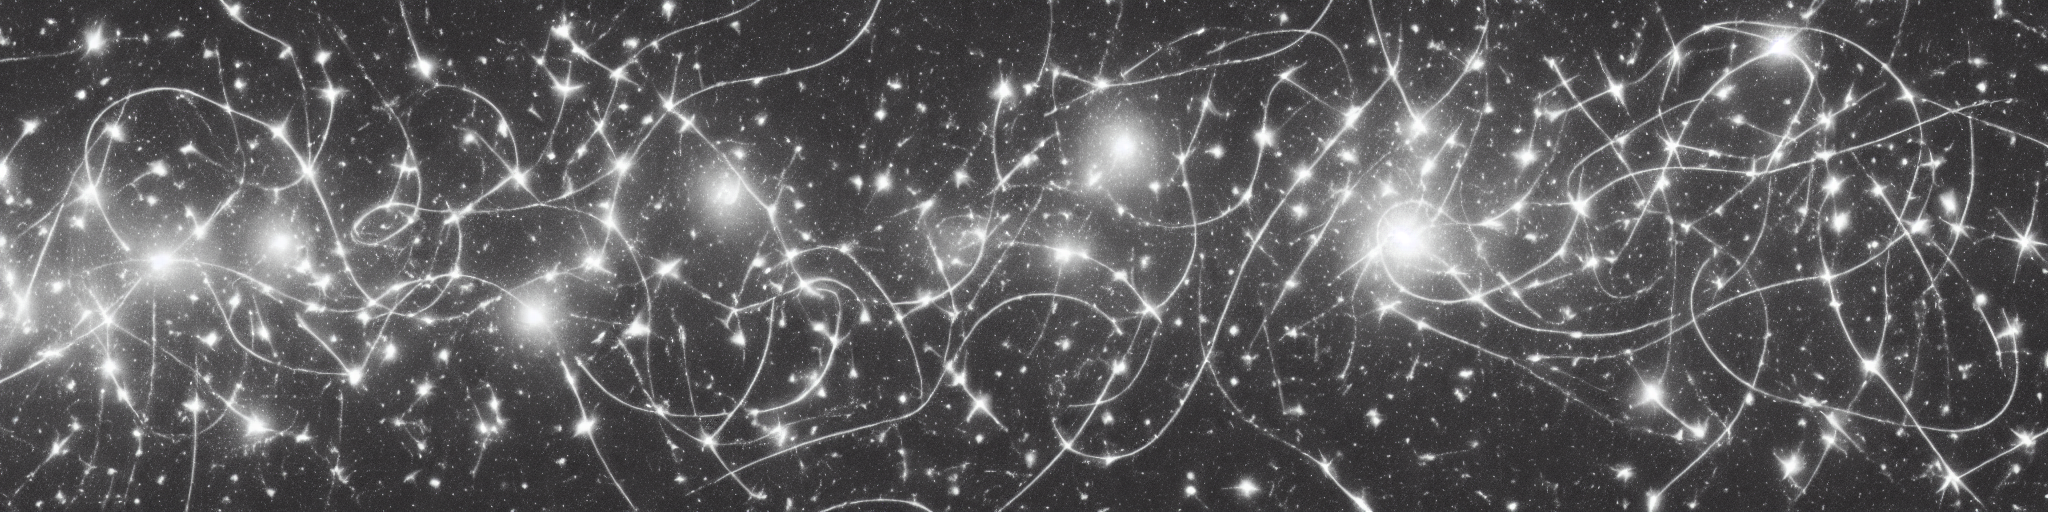
\includegraphics[width=1.18\paperwidth]{header2.png}%
% \transparent{0.16}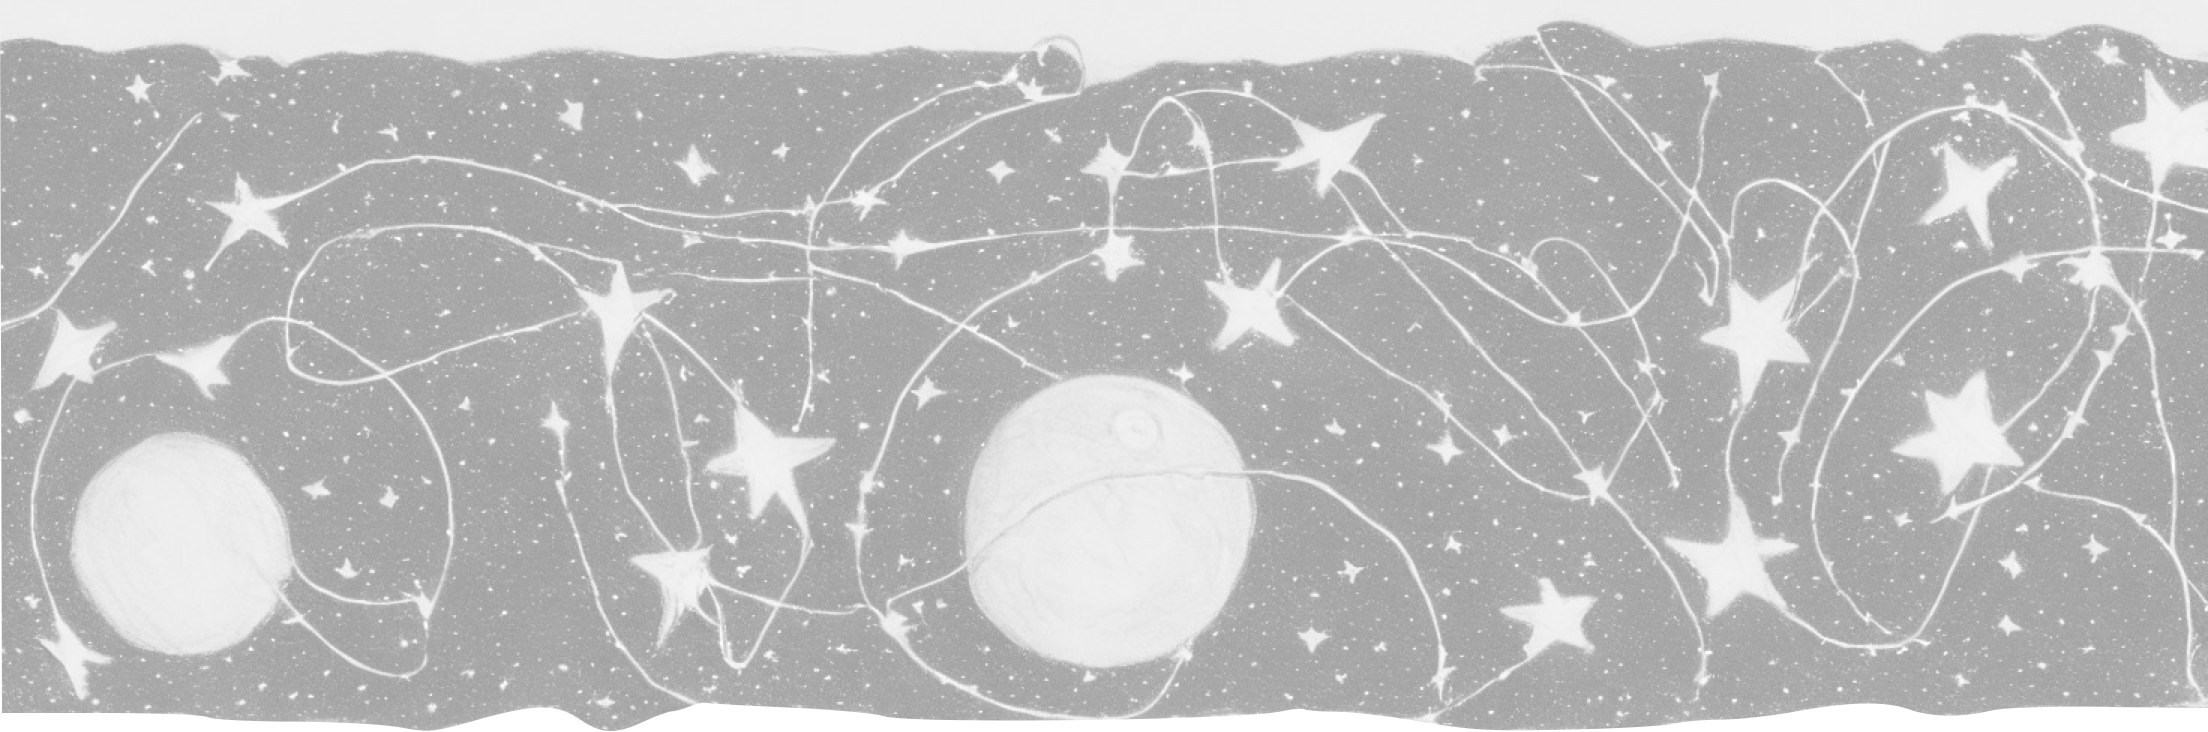
\includegraphics[width=1.04\paperwidth]{header.png}%
\vfill
}}}

\AddToShipoutPicture*{\BackgroundPic}

%%%%%%%%%%%%
% PDF setup

\ifpdf
  \usepackage[pdftex]{hyperref}
\else
  \usepackage[hypertex]{hyperref}
\fi
\hypersetup{
    letterpaper,
    colorlinks,
    linkcolor=linkcolor!\myshade!black,
    urlcolor=linkcolor!\myshade!black,
    pdfpagemode=none,
    pdftitle={Siddharth Mishra-Sharma's CV},
    pdfauthor={Siddharth Mishra-Sharma},
    pdfsubject={Siddharth Mishra-Sharma's CV},
    pdfkeywords={}
}

%%%%%%%%%%%%
% Toggle for printing phone number

% Get environmental variable ENV
\newcommand{\getenv}[2][]{%
  \CatchFileEdef{\temp}{"|kpsewhich --var-value #2"}{\endlinechar=-1}%
  \if\relax\detokenize{#1}\relax\temp\else\let#1\temp\fi}

\getenv[\ENV]{ENV}

% Print phone number ONLY if not compiling online GitHub version
\ifthenelse{\equal{\ENV}{GIT}}
  {
   \newcommand{\phone}{}%
  }
  {
   \newcommand{\phone}{~\lightsep~\faMobile\hspace{1mm}\href{tel:16099330103}{+1 (609) 933-0103}}%
  }
%%%%%%%%%%%%

%%%%%%%%%%%%
% Margin setup
\oddsidemargin=-0.4in
\evensidemargin=-0.4in
\textwidth=7.2in
\headheight=-0.6in
\topmargin=0.12in
\textheight=9.6in
%%%%%%%%%%%%

%% Setup the header and footer
\pagestyle{fancy}
\fancyhf{}
\cfoot{Page\ \thepage\ of\ \pageref*{LastPage}}
\renewcommand{\headrulewidth}{0pt}
\renewcommand{\footrulewidth}{0.8pt}

\setlength{\tabcolsep}{0in}
\hyphenchar\font=-1

% Change bullet size
\makeatletter
\renewcommand\@biblabel[1]{\textbullet}
\makeatother

% Packed itemize environment
\newenvironment{packed_itemize}{
\begin{itemize}[label=\raisebox{0.25ex}{\tiny$\bullet$}]
  \setlength{\itemsep}{4.2pt}
  \setlength{\parskip}{0pt}
  \setlength{\parsep}{0pt}}{\end{itemize}
}

% Packed enumerate environment
\newenvironment{packed_enumerate}[1][]{
\begin{etaremune}[#1]
  \setlength{\itemsep}{3.7pt}
  \setlength{\parskip}{0pt}
  \setlength{\parsep}{0pt}}{\end{etaremune}
}
 \fancypagestyle{style1}{
 \fancyhf{}
 \fancyhead[C]{style 1 with thin line}
 \fancyfoot[C]{\thepage}
 \renewcommand{\headrulewidth}{0.4pt}
 }


\newcommand{\SubItem}[1]{
    {\setlength\itemindent{15pt} \item[-] #1}
}

\begin{document}
\sloppy
\raggedbottom

%%%%%%%%%%%%
%% Heading

\begin{center}
\begin{tabular*}{\textwidth}{@{\extracolsep{\fill}}lcr}
&\huge{\textbf{\sc{Siddharth Mishra-Sharma}}}&   \\
& 77 Massachusetts Ave, 26-648, 
Cambridge, MA 02139, USA &\\

%&\faEnvelopeO\hspace{1mm}\href{mailto:smsharma@mit.edu}{\texttt{smsharma@mit.edu}} 
&\faEnvelopeO\hspace{1mm}\href{mailto:smsharma@mit.edu}{\texttt{smsharma@mit.edu}} 
\phone
~\lightsep~\faGlobe\hspace{1mm}\href{https://smsharma.io}{\texttt{smsharma.io}} 
~\lightsep~\faGithub\hspace{1mm}\href{https://github.com/smsharma}{\texttt{github.com/smsharma}} 
\vspace{0.5mm}
\\ 

\hline\hline

\end{tabular*}
\end{center}

\vspace{2.0mm}

%%%%%%%%%%%%

%%%%%%%%%%%%
%% Appointments 

\noindent
\begin{tabular*}{\textwidth}{l@{\extracolsep{\fill}}}
\large {\sc \Large{\faSuitcase~Appointments}}\\
\hline
\end{tabular*}

% Anthropic
\noindent 
\\
\begin{tabular*}{\textwidth}{l@{\extracolsep{\fill}}r}
\textbf{Anthropic} & \textbf {San Francisco, CA, USA}\\
\emph{Member of Technical Staff}  & {Nov. 2024 -- Present}\\
\emph{Resident}  & {Jul. 2024 -- Oct. 2024}\vspace{2mm}\\
\end{tabular*}

% BU
\noindent 
\\
\begin{tabular*}{\textwidth}{l@{\extracolsep{\fill}}r}
\textbf{Boston University} & \textbf {Boston, MA, USA}\\
\href{https://www.bu.edu/cds-faculty/profile/siddharth-mishra-sharma/}{Faculty of Computing \& Data Sciences}\\
\emph{Assistant Professor of Computing \& Data Sciences and Physics}  & {Starting in Jul. 2025} \\
\emph{Visiting Researcher}  & {Jun. 2024 -- Present}\vspace{2mm}\\
\end{tabular*}

% MIT
\noindent 
\\
\begin{tabular*}{\textwidth}{l@{\extracolsep{\fill}}r}
%\textbf{Massachusetts Institute of Technology}, \small{Center for Theoretical Physics}  & \textbf {Cambridge, MA, USA}\\
%\textbf{Harvard University}, \small{Department of Physics} & \textbf {Cambridge, MA, USA}\\
\textbf{Massachusetts Institute of Technology} & \textbf {Cambridge, MA, USA}\\
\textbf{Harvard University} & \textbf {Cambridge, MA, USA}\\
\href{https://iaifi.org/}{NSF AI Institute for Artificial Intelligence and Fundamental Interactions}\\
\emph{IAIFI Fellow}  & {Sep. 2021 -- Jul. 2024}\vspace{2mm}\\
\end{tabular*}

% NYU
\noindent 
\\
\begin{tabular*}{\textwidth}{l@{\extracolsep{\fill}}r}
\textbf{New York University} & \textbf {New York, NY, USA}\\
\href{http://www.ccpp.nyu.edu/index.php}{Center for Cosmology and Particle Physics}\\
\emph{Postdoctoral Associate}  & {Sep. 2018 -- Aug. 2021} \\  
\end{tabular*}
\vspace{2.0mm}

%%%%%%%%%%%%
%% Education 

\noindent
\begin{tabular*}{\textwidth}{l@{\extracolsep{\fill}}}
\large {\sc \Large{\faGraduationCap~Education}}\\
\hline
\end{tabular*}

% Princeton
\noindent 
\\
\begin{tabular*}{\textwidth}{l@{\extracolsep{\fill}}r}
\textbf{Princeton University}  & \textbf {Princeton, NJ, USA}\vspace{0mm}\\
{Ph.D. in Theoretical Physics}  & {Sep. 2013 -- Aug. 2018} \vspace{.0mm} \\  
{Thesis: \href{https://dataspace.princeton.edu/jspui/handle/88435/dsp012v23vx15d}{\emph{Extragalactic Searches for Dark Matter Annihilation}}}& {} \vspace{0mm} \\
{Advisor: Mariangela Lisanti}& {} \vspace{2mm} \\
% \small{M.A. awarded in Jan. 2015}& {} \vspace{2mm} \\

\end{tabular*}

% Cambridge
\noindent 
\\
\begin{tabular*}{\textwidth}{l@{\extracolsep{\fill}}r}
\textbf{University of Cambridge}  & \textbf {Cambridge, UK}\vspace{0mm}\\
{Part III of the Mathematical Tripos (M.Math.)} & {Oct. 2012 -- Jun. 2013}\vspace{0.0mm}\\ 
% \small{\emph{Specializing in Theoretical Physics}}\vspace{1mm}\\
{B.A. (Hons.) in Natural Sciences (Physical)} & {Oct. 2009 -- Jun. 2012} \\
% \small{\emph{Specializing in Physics}}\vspace{1mm}\\
\end{tabular*}
%\small{M.A. (Cantab) awarded in May 2016. \small{\emph{Note that this is an academic rank that may be given six years after the end of a first term at the University of Cambridge, and is not a postgraduate qualification.}}}\vspace{0mm}\\
\vspace{2.0mm}
%%%%%%%%%%%%

%%%%%%%%%%%%
%% Publications 

\noindent
\begin{tabular*}{\textwidth}{l@{\extracolsep{\fill}}r}
\large {\sc \Large{\faBook~Publications}} & 
\href{https://arxiv.org/a/mishrasharma_s_1.html}{\arxivlogo}  \
\href{https://scholar.google.com/citations?hl=en&user=hJVjhlwAAAAJ&view_op=list_works&sortby=pubdate}{\scholarlogo}  \ 
\href{https://inspirehep.net/authors/1394493}{\inspirelogo}  \ 
\href{https://ui.adsabs.harvard.edu/search/p_=0&q=author%3A%22Mishra-Sharma%2C%20Siddharth%22&sort=date%20desc%2C%20bibcode%20desc}{\adslogo} \\
\hline
\end{tabular*}\vspace{3.5mm}

\noindent
Primary contributions: \emph{(Note: where indicated with an asterisk\,$^*$, authors are listed in alphabetical order as per the standard in that field. $^{\dagger}$denotes equal contribution.)}

\begin{packed_enumerate}[start=48]

%- Simulate what you want
%- Overconfident NPTF
%- NPTF SVI
%- Evidences and biases
  
\item E.D. Ramirez, Y. Sun, M.R. Buckley, \underline{S. Mishra-Sharma}, T.R. Slatyer, \emph{Inferring the Morphology of the Galactic Center Excess with Gaussian Processes} \href{https://arxiv.org/abs/2410.21367}{[arXiv:2410.21367]}

\item J. Balla, \underline{S. Mishra-Sharma}, C. Cuesta-Lazaro, T. Jaakkola, T. Smidt, \emph{A Cosmic-Scale Benchmark for Symmetry-Preserving Data Processing}, Accepted at Proceedings of Machine Learning Research (PMLR) Volume on Symmetry and Geometry in Neural Representations; Accepted at Learning on Graphs Conference 2024 (Extended Abstract; {\textbf{Spotlight Oral}}) \href{https://arxiv.org/abs/2410.20516}{[arXiv:2410.20516]}

\item T. Nguyen, F. Villaescusa-Navarro, \underline{S. Mishra-Sharma} et al., \emph{How DREAMS are made: Emulating Satellite Galaxy and Subhalo Populations with Diffusion Models and Point Clouds}, Under review at Astrophys.J. \href{https://arxiv.org/abs/2409.02980}{[arXiv:2409.02980]}

\item $^{\dagger}$G. Zhang, $^{\dagger}$T. Helfer, A. Gagliano, \underline{S. Mishra-Sharma}, V.A. Villar, \emph{Maven: A Multimodal Foundation Model for Supernova Science}, Accepted at NeurIPS 2023 Foundation Models for Science Workshop, NeurIPS 2023 Workshop on Time Series in the Age of Large Models {\textbf{[Spotlight Oral]}}, NeurIPS 2024 Workshop on Self-Supervised Learning; Under review at Mach.Learn.Sci.Tech \href{https://arxiv.org/abs/2408.16829}{[arXiv:2408.16829]}

\item A. Delaunoy, M. de la Brassinne Bonardeaux, \underline{S. Mishra-Sharma}, G. Louppe, \emph{Low-Budget Simulation-Based Inference with Bayesian Neural Networks}, Under review at ICLR 2024 \href{https://arxiv.org/abs/2408.15136}{[arXiv:2408.15136]}

\item $^*$C. Giovanetti, M. Lisanti, H. Liu, \underline{S. Mishra-Sharma}, J.T. Ruderman, \emph{LINX: A Fast, Differentiable, and Extensible Big Bang Nucleosynthesis Package}, Under review at Phys.Rev. D \href{https://arxiv.org/abs/2408.14538}{[arXiv:2408.14538]}

  \item $^*$C. Giovanetti, M. Lisanti, H. Liu, \underline{S. Mishra-Sharma}, J.T. Ruderman, \emph{Cosmological Parameter Estimation with a Joint-Likelihood Analysis of the Cosmic Microwave Background and Big Bang Nucleosynthesis}, Under review at Phys.Rev.Lett. \href{https://arxiv.org/abs/2408.14531}{[arXiv:2408.14531]}

  \item N. Sabti, R. Reddy, J.B. Muñoz, \underline{S. Mishra-Sharma}, T. Youn, \emph{A Generative Modeling Approach to Reconstructing 21-cm Tomographic Data}, Under review at Mach.Learn.Sci.Tech \href{https://arxiv.org/abs/2407.21097}{[arXiv:2407.21097]}

  \item \underline{S. Mishra-Sharma}, Y. Song, J. Thaler, \emph{PAPERCLIP: Associating Astronomical Observations and Natural Language with Multi-Modal Models}, Accepted at \href{https://colmweb.org/}{Conference on Language Modeling (COLM 2024)}  \href{https://arxiv.org/abs/2403.08851}{[arXiv:2403.08851]}

  \item M.M. Ivanov, $^{\dagger}$C. Cuesta-Lazaro, $^{\dagger}$\underline{S. Mishra-Sharma}, $^{\dagger}$A. Obuljen, $^{\dagger}$M. Toomey, \emph{Full-shape analysis with simulation-based priors: constraints on single field inflation from BOSS}, Accepted at Phys.Rev. {D} \href{https://arxiv.org/abs/2402.13310}{[arXiv:2402.13310]}

  \item $^*$L. Heinrich, \underline{S. Mishra-Sharma}, C. Pollard, P. Windischhofer, \emph{Hierarchical Neural Simulation-Based Inference Over Event Ensembles}, \href{https://openreview.net/forum?id=Jy2IgzjoFH&referrer=%5BAuthor%20Console%5D(%2Fgroup%3Fid%3DTMLR%2FAuthors%23your-submissions)}{Transactions on Machine Learning Research (TMLR)} \href{https://arxiv.org/abs/2306.12584}{[arXiv:2306.12584]}

  \item $^{\dagger}$\underline{S. Mishra-Sharma}, $^{\dagger}$C. Cuesta-Lazaro, \emph{A point cloud approach to generative modeling for galaxy surveys at the field level}
  \begin{packed_itemize}
      \item  \href{https://journals.aps.org/prd/abstract/10.1103/PhysRevD.109.123531}{Phys.Rev. {D}} \href{https://arxiv.org/abs/2311.17141}{[arXiv:2311.17141]}
      \item {Machine Learning for Astrophysics Workshop at the Fortieth International Conference on Machine Learning (ICML 2023)} \href{https://ml4astro.github.io/icml2023/}{\textbf{[Spotlight Oral]}} \href{https://ml4astro.github.io/icml2023/assets/59.pdf}{[Paper]} 
       \end{packed_itemize}

  \item $^*$\underline{S. Mishra-Sharma}, T.R. Slatyer, Y. Sun, Y. Wu, \emph{Disentangling gamma-ray observations of the Galactic Center using differentiable probabilistic programming}, {Machine Learning for Astrophysics Workshop at the Fortieth International Conference on Machine Learning (ICML 2023)} \href{https://ml4astro.github.io/icml2023/}{\textbf{[Spotlight Oral]}} \href{https://ml4astro.github.io/icml2023/assets/52.pdf}{[Paper]}

  \item A. Akhmetzanova, \underline{S. Mishra-Sharma}, C. Dvorkin, \emph{Data Compression and Inference in Cosmology with Self-Supervised Machine Learning}
  \begin{packed_itemize}
      \item \href{https://doi.org/10.1093/mnras/stad3646}{Mon.Not.Roy.Astron.Soc. 527 (2023) 7459} \href{https://arxiv.org/abs/2308.09751}{[arXiv:2308.09751]}
      \item {Machine Learning for Astrophysics Workshop at the Fortieth International Conference on Machine Learning (ICML 2023)} \href{https://ml4astro.github.io/icml2023/assets/11.pdf}{[Paper]} 
       \end{packed_itemize}
      
  \item G. Zhang, \underline{S. Mishra-Sharma}, C. Dvorkin, \emph{Inferring subhalo effective density slopes from strong lensing observations with neural likelihood-ratio estimation}, \href{https://doi.org/10.1093/mnras/stac3014}{Mon.Not.Roy.Astron.Soc. 517 (2022) 4317} \href{https://arxiv.org/abs/2208.13796}{[arXiv:2208.13796]}

  \item T. Nguyen, \underline{S. Mishra-Sharma}, R. Williams, L. Necib, \emph{Uncovering dark matter density profiles in dwarf galaxies with graph neural networks}
  \begin{packed_itemize}
      \item {\href{https://journals.aps.org/prd/abstract/10.1103/PhysRevD.107.043015}{Phys.Rev. \textbf{D107} (2023) 043015}} \href{https://arxiv.org/abs/2208.12825}{[arXiv:2208.12825]}
      \item Machine Learning for Astrophysics Workshop at the Thirty-ninth International Conference on Machine Learning (ICML 2022) \href{https://ml4astro.github.io/icml2022/}{\textbf{[Spotlight Oral]}} \href{https://ml4astro.github.io/icml2022/assets/38.pdf}{[Paper]}
    \end{packed_itemize}
    
  \item \underline{S. Mishra-Sharma}, G. Yang, \emph{Strong Lensing Source Reconstruction Using Continuous Neural Fields}, {Machine Learning for Astrophysics Workshop at the Thirty-ninth International Conference on Machine Learning (ICML 2022)} \href{https://ml4astro.github.io/icml2022/}{\textbf{[Spotlight Oral]}} \href{https://arxiv.org/abs/2206.14820}{[arXiv:2206.14820]}
   
  % \item $^*$T. Nguyen, \underline{S. Mishra-Sharma} and L. Necib, \emph{Uncovering dark matter density profiles in dwarf galaxies with graph neural networks}, {Machine Learning for Astrophysics Workshop at the Thirty-ninth International Conference on Machine Learning (ICML 2022)} \textbf{[Spotlight Oral]} \href{https://ml4astro.github.io/icml2022/assets/38.pdf}{[Paper]}

  \item $^*$A. Caputo, H. Liu, \underline{S. Mishra-Sharma}, M. Pospelov, J.T. Ruderman, \emph{A Stimulating Explanation of the Extragalactic Radio Background}, \href{https://journals.aps.org/prd/abstract/10.1103/PhysRevD.107.123033}{Phys.Rev. \textbf{D107} (2023) 123033} \href{https://arxiv.org/abs/2206.07713}{[arXiv:2206.07713]}

  \item  \underline{S. Mishra-Sharma}, K. Cranmer, \emph{A neural simulation-based inference approach for characterizing the Galactic Center $\gamma$-ray excess}
    \begin{packed_itemize}
      \item {\href{https://journals.aps.org/prd/abstract/10.1103/PhysRevD.105.063017}{Phys.Rev. \textbf{D105} (2022) 063017} \href{https://arxiv.org/abs/2110.06931}{[arXiv:2110.06931]}}
      \item {Machine Learning and the Physical Sciences Workshop at the 35th Conference on Neural Information Processing Systems (NeurIPS 2021) \href{https://ml4physicalsciences.github.io/2020/files/NeurIPS_ML4PS_2020_20.pdf}{[Paper]}\,\href{https://ml4physicalsciences.github.io/2020/files/NeurIPS_ML4PS_2020_20_poster.pdf}{[Poster]}}
    \end{packed_itemize}

%  \item  $^*$\underline{S. Mishra-Sharma} and K. Cranmer, \emph{Characterizing $\gamma$-ray maps of the Galactic Center with neural density estimation}, Machine Learning and the Physical Sciences Workshop at the 35th Conference on Neural Information Processing Systems (NeurIPS 2021) \href{https://ml4physicalsciences.github.io/2020/files/NeurIPS_ML4PS_2020_20.pdf}{[Paper]}\,\href{https://ml4physicalsciences.github.io/2020/files/NeurIPS_ML4PS_2020_20_poster.pdf}{[Poster]}

  \item \underline{S. Mishra-Sharma}, \emph{Inferring dark matter substructure with astrometric lensing beyond the power spectrum}  
  \begin{packed_itemize}
    \item {\href{https://doi.org/10.1088/2632-2153/ac494a}{Mach.Learn.Sci.Tech. \textbf{3} (2022) 01LT03} \,\href{https://arxiv.org/abs/2110.01620}{[arXiv:2110.01620]}}
    \item {{Machine Learning and the Physical Sciences Workshop at the 35th Conference on Neural Information Processing Systems (NeurIPS 2021)} \href{https://ml4physicalsciences.github.io/2021/files/NeurIPS_ML4PS_2021_22_poster.png}{[Poster]}}
    \end{packed_itemize}

  \item\underline{S. Mishra-Sharma}, K. Cranmer, \emph{Semi-parametric $\gamma$-ray modeling with Gaussian processes and variational inference}, {Machine Learning and the Physical Sciences Workshop at the 34rd Conference on Neural Information Processing Systems (NeurIPS 2020)} \href{https://ml4physicalsciences.github.io/2020/files/NeurIPS_ML4PS_2020_20.pdf}{[Paper]}\,\href{https://ml4physicalsciences.github.io/2020/files/NeurIPS_ML4PS_2020_20_poster.pdf}{[Poster]}\,\href{https://arxiv.org/abs/2010.10450}{[arXiv:2010.10450]} 

  \item $^*$A. Caputo, H. Liu, \underline{S. Mishra-Sharma}, M. Pospelov, J.T. Ruderman, A. Urbano, \emph{Edges and Endpoints in 21-cm Observations from Resonant Photon Production},  \href{https://journals.aps.org/prl/abstract/10.1103/PhysRevLett.127.011102}{Phys.Rev.Lett. \textbf{127} (2021) 011102}   \href{https://arxiv.org/abs/2009.03899}{[arXiv:2009.03899]}

  \item J.J. Somalwar, L.J. Chang, \underline{S. Mishra-Sharma}, M. Lisanti, \emph{Harnessing the Population Statistics of Subhalos to Search for Annihilating Dark Matter}, \href{https://iopscience.iop.org/article/10.3847/1538-4357/abc87d}{Astrophys.J. \textbf{906} (2021) no.1, 57} \href{https://arxiv.org/abs/2009.00021}{[arXiv:2009.00021]}

  \item $^*$A. Caputo, H. Liu, \underline{S. Mishra-Sharma}, J.T. Ruderman, \emph{Modeling Dark Photon Oscillations in Our Inhomogeneous Universe}, \href{https://journals.aps.org/prd/abstract/10.1103/PhysRevD.102.103533}{Phys.Rev. \textbf{D102} (2020) 103533}   \href{https://arxiv.org/abs/2004.06733}{[arXiv:2004.06733]}

  \item \underline{S. Mishra-Sharma}, K. Van Tilburg, N. Weiner, \emph{Power of Halometry}, \href{https://journals.aps.org/prd/abstract/10.1103/PhysRevD.102.023026}{Phys.Rev. \textbf{D102} (2020) 023026} [\textbf{Editors' Suggestion} and \textbf{Featured} in \emph{Physics}; \href{https://physics.aps.org/articles/v13/s98}{Synopsis}]  \href{https://arxiv.org/abs/2003.02264}{[arXiv:2003.02264]}

  \item M. Buschmann, N.L. Rodd, B.R. Safdi, L.J. Chang, \underline{S. Mishra-Sharma}, M. Lisanti, O. Macias \emph{Foreground Mismodeling and the Point Source Explanation of the Fermi Galactic Center Excess},  \href{https://journals.aps.org/prd/abstract/10.1103/PhysRevD.102.023023}{Phys.Rev. \textbf{D102} (2020) 023023} \href{https://arxiv.org/abs/2002.12373}{[arXiv:2002.12373]} 

  \item $^*$A. Caputo, H. Liu, \underline{S. Mishra-Sharma}, J.T. Ruderman, \emph{Dark Photon Oscillations in Our Inhomogeneous Universe}, \href{https://journals.aps.org/prl/abstract/10.1103/PhysRevLett.125.221303}{Phys.Rev.Lett. \textbf{125} (2020) 221303}  \href{https://arxiv.org/abs/2002.05165}{[arXiv:2002.05165]}

  \item J. Brehmer, K. Cranmer, \underline{S. Mishra-Sharma}, F. Kling, G. Louppe, \emph{Mining gold: Improving simulation-based inference with latent information}, {Machine Learning and the Physical Sciences Workshop at the 33rd Conference on Neural Information Processing Systems (NeurIPS 2019)} \href{https://ml4physicalsciences.github.io/files/NeurIPS_ML4PS_2019_16.pdf}{[Paper]}

  \item $^{*\dagger}$J. Brehmer, $^\dagger$\underline{S. Mishra-Sharma}, J. Hermans, G. Louppe, K. Cranmer, \emph{Mining for Dark Matter Substructure: Inferring subhalo population properties from strong lenses with machine learning}, \href{https://iopscience.iop.org/article/10.3847/1538-4357/ab4c41}{Astrophys.J. \textbf{886} (2019) no.1, 49} \href{https://arxiv.org/abs/1909.02005}{[arXiv:1909.02005]}

  \item L.J. Chang, \underline{S. Mishra-Sharma}, M. Lisanti, M. Buschmann, N.L. Rodd, B.R. Safdi, \emph{Characterizing the Nature of the Unresolved Point Sources in the Galactic Center: An Assessment of Systematic Uncertainties},  \href{https://journals.aps.org/prd/abstract/10.1103/PhysRevD.101.023014}{Phys.Rev. \textbf{D101} (2020) 023014} \href{https://arxiv.org/abs/1908.10874}{[arXiv:1908.10874]}, 

  \item $^*$L.J. Chang, M. Lisanti, \underline{S. Mishra-Sharma}, \emph{Search for Dark Matter Annihilation in the Milky Way Halo}, \href{https://journals.aps.org/prd/abstract/10.1103/PhysRevD.98.123004}{Phys.Rev. \textbf{D98} (2018) 123004} \href{https://arxiv.org/abs/1804.04132}{[arXiv:1804.04132]}

  \item \underline{S. Mishra-Sharma}, D. Alonso, J. Dunkley, \emph{Neutrino masses and beyond-$\Lambda$CDM cosmology with LSST and future CMB experiments}, \href{https://journals.aps.org/prd/abstract/10.1103/PhysRevD.97.123544}{Phys.Rev. \textbf{D97} (2018) 123544}  \href{https://arxiv.org/abs/1803.07561}{[arXiv:1803.07561]}

  \item $^*$R. Bartels, D. Hooper, T. Linden, \underline{S. Mishra-Sharma}, N.L. Rodd, B.R. Safdi, T.R. Slatyer, \emph{Comment on ``Characterizing the population of pulsars in the Galactic bulge with the
  {\it Fermi} Large Area Telescope'' [arXiv:1705.00009\MakeLowercase{v}1]}, \href{https://www.sciencedirect.com/science/article/pii/S2212686418300268}{Phys.Dark Univ. \textbf{20} (2018) 88-94} \href{https://arxiv.org/abs/1710.10266}{[arXiv:1710.10266]}

  \item $^*$M. Lisanti, \underline{S. Mishra-Sharma}, N.L. Rodd, B.R. Safdi, \emph{Mapping Extragalactic Dark Matter Annihilation with Galaxy Surveys: A Systematic Study of Stacked Group Searches},  \href{https://journals.aps.org/prd/abstract/10.1103/PhysRevD.97.063005}{Phys.Rev. \textbf{D97} (2018) 063005} \href{https://arxiv.org/abs/1709.00416}{[arXiv:1709.00416]}

  \item $^*$M. Lisanti, \underline{S. Mishra-Sharma}, N.L. Rodd, B.R. Safdi, \emph{Search for Dark Matter Annihilation in Galaxy Groups},  \href{https://journals.aps.org/prl/abstract/10.1103/PhysRevLett.120.101101}{Phys.Rev.Lett. \textbf{120} (2018) 101101} \href{https://arxiv.org/abs/1708.09385}{[arXiv:1708.09385]}

  \item $^*$T. Cohen, M. Lisanti, H. K. Lou, \underline{S. Mishra-Sharma}, \emph{LHC Searches for Dark Sector Showers},  \href{https://link.springer.com/article/10.1007/JHEP11(2017)196}{JHEP \textbf{11}, 196 (2017)}  \href{https://arxiv.org/abs/1707.05326}{ [arXiv:1707.05326]}

  \item $^*$\underline{S. Mishra-Sharma}, N.L. Rodd, B.R. Safdi, \emph{NPTFit: A code package for Non-Poissonian Template Fitting},  \href{http://iopscience.iop.org/article/10.3847/1538-3881/aa6d5f/meta}{Astron.J. \textbf{153} (2017) no.6, 253}  \href{https://arxiv.org/abs/1612.03173}{ [arXiv:1612.03173]}

  \item $^*$Y. Kahn, G. Krnjaic, \underline{S. Mishra-Sharma}, T.M.P. Tait, \emph{Light Weakly Coupled Axial Forces: Models, Constraints, and Projections},  \href{https://link.springer.com/article/10.1007%2FJHEP05%282017%29002}{JHEP \textbf{05}, 002 (2017)}  \href{https://arxiv.org/abs/1609.09072}{[arXiv:1609.09072]}

  \item $^*$M. Lisanti, \underline{S. Mishra-Sharma}, L. Necib, B.R. Safdi, \emph{Deciphering Contributions to the Extragalactic Gamma-Ray Background from 2 GeV to 2 TeV},  \href{http://iopscience.iop.org/article/10.3847/0004-637X/832/2/117/meta}{Astrophys.J. \textbf{832} (2016) no.2, 117} \href{https://arxiv.org/abs/1606.04101}{[arXiv:1606.04101]}

  \item $^*$S.K. Lee, M. Lisanti, \underline{S. Mishra-Sharma}, B.R. Safdi, \emph{Modulation Effects in Dark Matter-Electron Scattering Experiments}, \href{https://journals.aps.org/prd/abstract/10.1103/PhysRevD.92.083517}{Phys.Rev. \textbf{D92} (2015) 083517} \href{https://arxiv.org/abs/1508.07361}{[arXiv:1508.07361]}
\end{packed_enumerate}

\noindent
Contributions to white papers and as part of larger collaborations:

\begin{packed_enumerate}[start=8]

\item G. Grosso, P. Harris, \underline{S. Mishra-Sharma}, P. Shanahan, \emph{A Virtuous Cycle: Generative AI and Discovery in the Physical Sciences}, \href{https://doi.org/10.21428/e4baedd9.70ae2021}{An MIT Exploration of Generative AI (2024)}

  \item C. Dvorkin, \underline{S. Mishra-Sharma} \emph{et al.}, \emph{Machine Learning and Cosmology: Snowmass 2021 White Paper} \href{https://arxiv.org/abs/2203.08056}{[arXiv:2203.08056]}

  \item K. Boddy \emph{et al.} (including \underline{S. Mishra-Sharma}), \emph{Snowmass2021 theory frontier white paper: Astrophysical and cosmological probes of dark matter},  \href{https://www.sciencedirect.com/science/article/pii/S2214404822000349}{J.HEAp 35 (2022) 112-138}  \href{https://arxiv.org/abs/2203.08056}{[arXiv:2203.08056]}

  \item R. Leane \emph{et al.} (including \underline{S. Mishra-Sharma}), \emph{Snowmass2021 Cosmic Frontier White Paper: Puzzling Excesses in Dark Matter Searches and How to Resolve Them} \href{https://arxiv.org/abs/2203.06859}{[arXiv:2203.06859]}

  \item J. Alimena \emph{et al.} (including \underline{S. Mishra-Sharma}), \emph{Searching for long-lived particles beyond the Standard Model at the Large Hadron Collider}, \href{https://iopscience.iop.org/article/10.1088/1361-6471/ab4574}{J.Phys.G 47 (2020) 090501} \href{https://arxiv.org/abs/1903.04497}{[arXiv:1903.04497]}

  \item S. Algeri \emph{et al.} (including \underline{S. Mishra-Sharma}), \emph{Statistical challenges in the search for dark matter} \href{https://arxiv.org/abs/1807.09273}{[arXiv:1807.09273]}

  \item DarkSide Collaboration (including \underline{S. Mishra-Sharma}), \emph{Constraints on Sub-GeV Dark Matter-Electron Scattering from the DarkSide-50 Experiment}, \href{https://journals.aps.org/prl/abstract/10.1103/PhysRevLett.121.111303}{Phys.Rev.Lett. \textbf{121} (2018) 111303} \href{https://arxiv.org/abs/1802.06998}{[arXiv:1802.06998]}

  \item DarkSide Collaboration (including \underline{S. Mishra-Sharma}), \emph{Low-Mass Dark Matter Search with the DarkSide-50 Experiment}, \href{https://journals.aps.org/prl/abstract/10.1103/PhysRevLett.121.081307}{Phys.Rev.Lett. \textbf{121} (2018) 081307}  \href{https://arxiv.org/abs/1802.06994}{[arXiv:1802.06994]}
\end{packed_enumerate}
\vspace{2.0mm}

%%%%%%%%%%%%

%%%%%%%%%%%%
%% Talks 

\noindent
\begin{tabular*}{\textwidth}{l@{\extracolsep{\fill}}}
\large {\sc \Large{\faBullhorn~Seminars, Colloquia, and Conference Talks}}\\
\hline
\end{tabular*}\vspace{3.5mm}

\noindent
Invited talks:
\begin{packed_itemize}
  \item UC Santa Barbara Computer Science Colloquium \hfill Santa Barbara, CA, Jun. 2024
  \item KITP Program: Cosmic Signals of Dark Matter Physics \hfill Santa Barbara, CA, Jun. 2024
  \item European AI for Fundamental Physics Conference, Plenary \hfill Amsterdam, Netherlands, Apr. 2024
  \item Herzberg Astronomy and Astrophysics Research Centre Colloquium (Remote) \hfill Apr. 2024
  \item Rutgers High Energy Theory Seminar \hfill New Brunswick, NJ, Mar. 2024
  \item Boston University Computing \& Data Sciences (CDS) Colloquium \hfill Boston, MA, Feb. 2024
  \item Georgia Tech School of Physics Colloquium \hfill Atlanta, GA, Jan. 2024
  \item Rising Stars in Data Science Workshop \hfill Chicago, IL, Nov. 2023
  \item Summit for AI Institutes Leadership \hfill Atlanta, GA, Oct. 2023
  \item Johns Hopkins University Cosmology and Particle Physics Seminar \hfill Baltimore, MD, Oct. 2023
  \item MIAPbP Workshop on Differentiable and Probabilistic Programming \hfill Munich, Germany, Jun. 2023
  \item Status of the Galactic Center Excess Workshop \hfill New Brunswick, NJ, Jun. 2023
  \item Simons Foundation MATH+X Symposium \hfill Hella, Iceland, May. 2023
  \item Cosmic Connections: ML X Astrophysics (Flatiron Institute) \hfill New York, NY, May. 2023
  \item Harvard Center for Astrophysics ITC Lunch Talk  \hfill Cambridge, MA, Apr. 2023
  \item Aspen Center for Physics Winter Session \hfill Aspen, CO, Mar. 2023
  \item Normal Computing (Probabilistic AI Startup; Remote) \hfill Feb. 2023
  \item Yale Astronomy Colloquium \hfill New Haven, CT, Feb. 2023
  \item Mila ML for the Physical Sciences Reading Group \hfill Montr\'eal, Quebec, Jan. 2023
  \item McGill Space Institute Astronomy Seminar \hfill Montr\'eal, Quebec, Jan. 2023
  \item Nature of Dark Matter on Small Scales Meeting (Remote) \hfill  Oct. 2022
  \item Dagstuhl Seminar: Bridging Data-driven and Mechanistic Modelling \hfill Dagstuhl, Germany, Sep. 2022
  \item Hammers \& Nails Workshop 2022 \hfill Rehovot, Israel, Aug. 2022
  \item ICML 2022 ML4Astro Workshop (Spotlight oral) \hfill Baltimore, MD, May. 2022
  \item Physics $\cap$ ML Seminar (Remote at \href{http://www.physicsmeetsml.org//}{\texttt{physicsmeetsml.org}}) \hfill May. 2022
  \item Harvard CHASC Astrostatistics Seminar (Remote)  \hfill Apr. 2022
  \item University of Illinois Urbana-Champaign Phenomenology Seminar  \hfill Urbana, IL, Mar. 2022
  \item Harvard High Energy Theory Seminar \hfill Cambridge, MA, Mar. 2022
  \item American Astronomical Society 239th Meeting (Invited panel)  \hfill Salt Lake City, UT, Jan. 2022
  \item Harvard LPPC (High Energy Experiment) Seminar \hfill Cambridge, MA, Nov. 2021
  \item Rutgers High Energy Theory Seminar \hfill New Brunswick, NJ, Oct. 2021
  \item Instituto de Astrof\'{i}sica de Canarias Astrophysics Seminar (Remote) \hfill Sep. 2021
  \item Stony Brook University YITP Seminar (Remote) \hfill Mar. 2021
  \item SLAC AI Seminar Series (Remote) \hfill Feb. 2021
  \item Northeastern University Physics Colloquium (Remote) \hfill Feb. 2021
  \item Carnegie Observatories ``Lunch Talk'' Seminar (Remote) \hfill Feb. 2021
  \item BSM PANDEMIC Seminar  (Remote at \href{https://www.bsmpandemic.com/}{\texttt{bsmpandemic.com}}) \hfill Nov. 2020
  \item SLAC Elementary Particle Physics Seminar (Remote) \hfill Jul. 2020
  \item University of Amsterdam GRAPPA Colloquium (Remote) \hfill May 2020
  \item Princeton Pheno \& Vino Seminar (Remote) \hfill Apr. 2020
  \item CERN-TH BSM Forum (Remote) \hfill  Apr. 2020
  \item Machine Learning for Astrophysicists Seminar (Remote at \href{https://docs.google.com/document/d/1GGtE-YIuAWlmpKSr38_kyiF-Fklszhkh4FkiYWzBAho/pub}{\texttt{mlclub.net}}) \hfill  Mar. 2020
  \item University of Michigan LCTP Brown Bag Seminar \hfill Ann Arbor, MI, Jan. 2020
  \item Stony Brook University Particle Physics Seminar \hfill Stony Brook, NY, Nov. 2019
  \item Minnesota High Energy Theory Lunchtime Seminar \hfill  Minneapolis, MN, Nov. 2019
  \item Brown Astrophysics Seminar Series \hfill Providence, RI, May 2019
  \item Particles, Strings and Cosmology (PASCOS) 2018 \hfill Cleveland, OH, Jun. 2018
  \item Recontres de Blois 2018 \hfill Blois, France, Jun. 2018
  \item Princeton Astrophysics/IAS Cosmology Lunch Seminar \hfill Princeton, NJ, May 2018
  \item Fermilab Particle Astrophysics Seminar \hfill Batavia, IL, Mar. 2018
  \item Workshop on Statistical Challenges in the Search for Dark Matter \hfill Banff, Canada, Feb. 2018
  \item Maryland Elementary Particle Theory Seminar \hfill College Park, MD, Nov. 2017
  \item Rutgers High Energy Theory Seminar \hfill New Brunswick, NJ, Nov. 2017
  \item Cornell Particle Theory Seminar \hfill Ithaca, NY, Nov. 2017
  \item Caltech Particle Theory Seminar \hfill Pasadena, CA, Oct. 2017
  \item UC Irvine Joint Particle Seminar \hfill Irvine, CA, Oct. 2017
  \item ICTP LHC Long-Lived Particles Community Workshop (Remote) \hfill Oct. 2017
  \item Oxford Dalitz Seminar in Fundamental Physics  \hfill Oxford, UK, Oct. 2017
  \item KIPAC Tea Talk  \hfill Stanford, CA, Sep. 2017
  \item UC Santa Cruz Institute for Particle Physics Seminar  \hfill Santa Cruz, CA, Sep. 2017
  \item Berkeley 4D Seminar  \hfill Berkeley, CA, Sep. 2017
  \item MIT BSM Journal Club \hfill Boston, MA, Nov. 2016
\end{packed_itemize}

\noindent
Internal talks:
\begin{packed_itemize}
  \item MIT Physics Large Language Models Workshop \hfill Cambridge, MA, Jul. 2023
  \item IAIFI Seminar \hfill Cambridge, MA, Apr. 2022
  \item MIT CTP Nuclear and Particle Theory Seminar \hfill Cambridge, MA, Feb. 2022
  \item MIT CTP Graduate Student Lunch Seminar (Remote) \hfill Mar. 2021
  \item MIT QCD-DM-BSM-LHC Journal Club (Remote) \hfill Mar. 2021
  \item NYU CCPP Brown Bag Seminar \hfill New York, NY, Apr. 2019
  \item Princeton Pheno \& Vino Seminar \hfill Princeton, NJ, Apr. 2017
\end{packed_itemize}

\noindent
Contributed talks:
\begin{packed_itemize}
  \item 1st Large Language Models in Physics Symposium (LIPS)  \hfill Hamburg, Germany, Feb. 2024
  \item MIT Statistics and Data Science Conference  \hfill Cambridge, MA, Apr. 2022
  \item WFIRST Science Meeting (Flatiron Institute) \hfill New York, NY, Mar. 2020
  \item LSST Dark Matter Workshop \hfill Chicago, IL, Aug. 2019
  \item SUSY 2019 \hfill Corpus Christi, TX, May 2019
  \item Phenomenology Symposium (Pheno) 2019 \hfill Pittsburgh, PA, May 2019
  \item Dark Matter, Neutrinos and their Connection (DA$\nu$CO) \hfill Odense, Denmark, Aug. 2017
  \item TeV Particle Astrophysics (TeVPA) 2017 \hfill Columbus, OH, Aug. 2017 
  \item Phenomenology Symposium (Pheno) 2017 \hfill Pittsburgh, PA, May 2017 
  \item APS April Meeting 2017 \hfill Washington, DC, Jan. 2017 
  \item TeV Particle Astrophysics (TeVPA) 2016 \hfill Geneva, Switzerland, Sep. 2016 
  \item Gamma Rays and Dark Matter Workshop \hfill Obergurgl, Austria, Dec. 2015
  \item Phenomenology Symposium (Pheno) 2015 \hfill Pittsburgh, PA, May 2015
\end{packed_itemize}
\vspace{2.0mm}

%%%%%%%%%%%%

%%%%%%%%%%%%
%% Prizes and Honours 

\noindent
\begin{tabular*}{\textwidth}{l@{\extracolsep{\fill}}}
\large {\sc \Large{\faTrophy~Awards and Honors}}\\
\hline
\end{tabular*}\vspace{1.mm}

\begin{packed_itemize}
  \item \href{https://datascience.uchicago.edu/research/postdoctoral-programs/rising-stars-in-data-science-2/2023-rising-stars/}{Rising Stars in Data Science}, \emph{University of Chicago DSI and UCSD HDSI} \hfill 2023 \\ \emph{\small Focuses on celebrating and fast tracking the careers of exceptional data scientists at a critical \\ inflection point in their career}
  \item \href{https://iaifi.org/current-fellows.html}{IAIFI Fellowship} \hfill 2021 \\ \emph{\small Awarded towards independent postdoctoral research at the intersection of physics and artificial intelligence}
  \item Department Teaching Award, \emph{Princeton Department of Physics}  \hfill 2018 \\ \emph{\small Awarded for excellence in the role of Assistant in Instruction for courses taught at Princeton}
  \item Kusaka Memorial Prize in Physics, \emph{Princeton Department of Physics} \hfill 2017 \\ \emph{\small Awarded to physics graduate students who have shown outstanding performance in research \\ and professional promise}
  \item Princeton Graduate School Impact Award, \emph{Princeton Graduate School} \hfill 2016 \\ \emph{\small Awarded to an individual in the community that has made a difference during their time at Princeton}
  \item Princeton First-Year Graduate Fellowship, \emph{Princeton University} \hfill 2013 \\ \emph{\small Awarded towards the first year of graduate study at Princeton}
  \item Hugo de Balsham Prize, \emph{Peterhouse, University of Cambridge}  \hfill 2012 \\ \emph{\small Awarded for exceptional academic distinction at Peterhouse, Cambridge}
  \item Peter Scheuer Scholarship in Natural Sciences, \emph{Peterhouse, University of Cambridge} \hfill 2011, 2012 \\ \emph{\small Awarded for exceptional academic performance in the Cambridge second and third year Tripos examinations}
  \item Senior Academic Scholarship, \emph{Peterhouse, University of Cambridge} \hfill 2010\\ \emph{\small Awarded for exceptional academic performance in the Cambridge first year Tripos examinations}
\end{packed_itemize}
\vspace{2.0mm}

%%%%%%%%%%%%

%%%%%%%%%%%%
%% Broader impact
 
\noindent
\begin{tabular*}{\textwidth}{l@{\extracolsep{\fill}}}
\large {\sc \Large{\faUsers~Broader Impact and Organizing}}\\
\hline
\end{tabular*}\vspace{3.5mm}

\noindent
External organizing:
\begin{packed_itemize}
\item \noindent\begin{minipage}[t]{0.84\linewidth}
      \emph{Organizer}, \href{https://www.munich-iapbp.de/}{MIAPbP Program}: 
      \emph{\href{https://www.munich-iapbp.de/activities/activities-2025/machine-learning}{Build Big or Build Smart: Examining Scale and Domain Knowledge in Machine Learning for Fundamental Physics}}
      \end{minipage}%
      \begin{minipage}[t]{0.15\linewidth}
      \begin{flushright}
      2025
      \end{flushright}
      \end{minipage}\vspace{1.5mm}
\item \noindent\begin{minipage}[t]{0.84\linewidth}
      \emph{Organizer}, \href{https://aspenphys.org/summer-workshops/#event2401}{Aspen Center for Physics Summer Program}: 
      \emph{Fundamental Physics in the Era of Big Data and Machine Learning}
      \end{minipage}%
      \begin{minipage}[t]{0.15\linewidth}
      \begin{flushright}
      2024
      \end{flushright}
      \end{minipage}\vspace{1.5mm}
\item \noindent\begin{minipage}[t]{0.79\linewidth}
      \emph{Organizer}, \href{https://ml4physicalsciences.github.io/}{NeurIPS Machine Learning and the Physical Sciences Workshop}
      \end{minipage}%
      \begin{minipage}[t]{0.2\linewidth}
      \begin{flushright}
      2022, 2023, 2024
      \end{flushright}
      \end{minipage}  % \vspace{1.5mm}

\end{packed_itemize}

  \noindent
Internal organizing:
  \begin{packed_itemize}
  \item \emph{Organizer}, \href{https://iaifi.org/generative-ai-workshop}{Symposium on the Impact of Generative AI in the Physical Sciences}  \hfill 2024
  \item \emph{Organizer}, \href{https://iaifi.org/hackathon.html}{Boston-Area Machine Learning $\times$ Astrophysics Hackathon}  \hfill 2024
  \item \emph{Co-chair}, IAIFI Speaker Selection Committee  \hfill 2023 -- 2024
  \item \emph{Member}, IAIFI Computing Committee  \hfill 2022 -- 2024
  \item \emph{Member}, IAIFI Early Career and Equity Committee  \hfill 2021 -- 2023
  \item \emph{Organizer}, NYU CCPP Particle Physics Seminar \hfill 2019 -- 2020
  % \item \emph{Member}, Princeton University Student Life Committee \hfill 2016 -- 2018
  % \item \emph{Member}, Princeton Graduate Housing Advisory Board \hfill 2016 -- 2018
  \item \emph{Vice Chair}, Princeton Graduate College House Committee \hfill 2016 -- 2018
  \item \emph{Subject Representative}, Princeton Graduate Student Government Assembly \hfill 2013 -- 2017
  \item \emph{Organizer}, Princeton Physics Department Open House Committee  \hfill 2015 -- 2016
  \item \emph{Chair}, Princeton Physics Graduate Student Council \hfill 2015 -- 2018
\end{packed_itemize}
  \noindent
Reviewing/Editorial/Advisory:
  \begin{packed_itemize}
  \item \emph{Editorial Board}, Machine Learning: Science and Technology (MLST) \hfill 2024 -- Present
%  \item \emph{Advisory Board}, UKRI Center for Doctoral Training in AI for Decision Making in Complex Systems (Universities of Cambridge and Manchester) \hfill 2024 -- Present
  \item \emph{Journal Reviewer}, \ \scriptsize{Astrophysical Journal, Physical Review {D}, Physical Review {Letters}, Computer Physics Communications, JHEP,  JCAP, Journal of Open Source Software, MLST, MNRAS, Nature Communications Physics}\normalsize
    \item \emph{Conference Reviewer}, \scriptsize{NeurIPS Workshop Selection (2023, 2024), ICML Workshop Selection (2024), ICLR (2024)}\normalsize
  \item \emph{Workshop Reviewer},  \scriptsize{NeurIPS Machine Learning and the Physical Sciences Workshop (2019--2024), NeurIPS/ICML AI for Science Workshop (2021--2024), NeurIPS GenBio Workshop (2023), ICLR Workshop on Deep Generative Models for Highly Structured Data (2022), ICLR Workshop on Neural Fields (2023), ICML Workshop on Machine Learning for Astrophysics (2022, 2023), ICML Workshop on Structured Probabilistic Inference \& Generative Modeling (2023, 2024), ICML Workshop on Synergy of Scientific and Machine Learning Modeling (2023), ICML Differentiable Almost Everything Workshop (2024),  Advances in Approximate Bayesian Inference (2024)}\normalsize
  \item \emph{Grant Reviewer}, Department of Energy ASCR Leadership Computing Challenge \hfill 2023
  \item \emph{Grant Review Panelist}, NASA ROSES/Astrophysics Research and Analysis \hfill 2023
  
  \end{packed_itemize}
\vspace{2.0mm}

%%%%%%%%%%%%

%%%%%%%%%%%%
%% Mentoring 

\noindent
\begin{tabular*}{\textwidth}{l@{\extracolsep{\fill}}}
\large {\sc \Large{\faMagic~Research Mentorship}}\\
\hline
\end{tabular*}\vspace{1.mm}

\begin{packed_itemize}
  \item Yitian Sun (Graduate, {MIT Physics}) \hfill 2021 -- 2024 \\ \emph{Probabilistic programming and deep generative modeling for $\gamma$-ray data analysis}  \href{https://ml4astro.github.io/icml2023/assets/52.pdf}{[Paper]}
  \item Aizhan Akhmetzhanova (Graduate, {Harvard Physics}) \hfill 2021 -- 2024 \\ \emph{Simulation-based self-supervision for cosmological data analysis} \href{https://arxiv.org/abs/2308.09751}{[arXiv:2308.09751]}
  \item Tri Nguyen (Graduate, {MIT Astrophysics}) \hfill 2021 -- 2024 \\ \emph{Inferring the shapes of dark matter halos with graph neural networks} \href{https://arxiv.org/abs/2208.12825}{[arXiv:2208.12825]}
  \item Gemma Zhang (Graduate, {Harvard Physics}) \hfill 2021 -- 2024 \\ \emph{Inferring subhalo populations in strong lenses with likelihood-free inference} \href{https://arxiv.org/abs/2208.13796}{[arXiv:2208.13796]} \\ \emph{Multi-modal representation learning for time-domain astronomy}  \href{https://arxiv.org/abs/2408.16829}{[arXiv:2408.16829]}  \item Julia Balla (Graduate, {MIT EECS}) \hfill 2023 -- 2024 \\ \emph{Designing symmetry-preserving neural networks for cosmological data analysis}
  \item Julia Balla (Graduate, {MIT EECS}) \hfill 2023 -- 2024 \\ \emph{Designing symmetry-preserving neural networks for cosmological data analysis}
    \item Yiding Song (Harrow School; {MIT} via \href{https://www.cee.org/programs/research-science-institute}{Research Science Institute}) \hfill 2023 -- 2024 \\ \emph{Designing multi-modal language models for scientific data} \href{https://arxiv.org/abs/2403.08851}{[arXiv:2403.08851]}
  \item Reuel Williams (Undergraduate, {Princeton})\hfill 2021 \\ \emph{Inferring the shapes of dark matter halos with graph neural networks} \href{https://arxiv.org/abs/2208.12825}{[arXiv:2208.12825]}
  \item Jean Somalwar (Undergraduate, {Princeton})\hfill 2019 -- 2020 \\ \emph{Searching for dark matter in Galactic subhalos using photon statistics} \href{https://arxiv.org/abs/2009.00021}{[arXiv:2009.00021]}
  \item Laura Chang (Graduate, {Princeton})\hfill 2018 -- 2020 \\ \emph{Searches for annihilating dark matter in the Milky Way} \href{https://arxiv.org/abs/1804.04132}{[arXiv:1804.04132]}\,\href{https://arxiv.org/abs/1908.10874}{[arXiv:1908.10874]}
  \end{packed_itemize}
\vspace{2.0mm}

%%%%%%%%%%%%

%%%%%%%%%%%%
%% Teaching 

\noindent
\begin{tabular*}{\textwidth}{l@{\extracolsep{\fill}}}
\large {\sc \Large{\faWpforms~Teaching Experience}}\\
\hline
\end{tabular*}\vspace{3.5mm}

\noindent
At MIT/IAIFI:
\begin{packed_itemize}
  \item IAIFI Summer School \href{https://smsharma.io/iaifi-summer-school-2023/}{[Lectures on Generative Modeling]} \hfill Summer 2023
  \item 8.16 Data Science in Physics \href{https://github.com/smsharma/sbi-lecture-mit}{[Guest Lecture]} \hfill Spring 2023, Spring 2024
  \item IAIFI Summer School \href{https://github.com/smsharma/iaifi-summer-school-tutorials}{[Tutorials on Probabilistic Programming]} \hfill Summer 2022
  \item 8.S50 Computational Data Science in Physics \href{https://github.com/smsharma/prob-prog-8.S50-tutorial}{[Tutorials]} \hfill Winter 2022
\end{packed_itemize}

\noindent
At Princeton (As Assistant in Instruction):  {\scriptsize PHY235 Introduction to Research in Physics (Spring 2018), PHY312 Experimental Physics (Spring 2018), PHY115 Physics for Future Leaders (Fall 2017), PHY104 General Physics II (Spring 2016), PHY406 Nuclear and Elementary Particle Physics (Fall 2015), PHY106 Advanced Physics: Electromagnetism (Spring 2015), MAT201 Calculus III: Multivariable Calculus (Fall 2014, 2015), PHY105 Advanced Physics: Mechanics (Fall 2014)} \\

%\begin{packed_itemize}
%  \item PHY235 Introduction to Research in Physics \hfill Spring 2018
%  \item PHY312 Experimental Physics \hfill Spring 2018
%  \item PHY115  Physics for Future Leaders \hfill Fall 2017
%  \item PHY104  General Physics II \hfill Spring 2016
%  \item PHY406 Nuclear and Elementary Particle Physics \hfill Fall 2015
%  \item PHY106 Advanced Physics (Electromagnetism) \hfill Spring 2015
%  \item MAT201 Calculus III (Multivariable Calculus) \hfill Fall 2014, 2015
%  \item PHY105 Advanced Physics (Mechanics) \hfill Fall 2014
%\end{packed_itemize}
%\vspace{2.0mm}

%%%%%%%%%%%%

%%%%%%%%%%%%%
%%% Schools and Workshops
%
%\noindent
%\begin{tabular*}{\textwidth}{l@{\extracolsep{\fill}}}
%\large {\sc \Large{Workshops and Schools}}\\
%\hline
%\end{tabular*}\vspace{1.mm}
%
%\begin{packed_itemize}
%  \item \emph{Gaia} Sprint 2019 \hfill Santa Barbara, CA, Mar. 2019
%  \item Accelerating the Search for Dark Matter with Machine Learning \hfill Leiden, Netherlands, Jan. 2018
%  \item Prospects in Theoretical Physics (PiTP) \hfill Princeton, NJ, Jul. 2017
%  \item Theoretical Advanced Study Institute (TASI) \hfill Boulder, CO, Jun. 2016
%  \item Tri-Institute Summer School on Elementary Particles (TRISEP) \hfill Waterloo, Canada, Jul. 2015
%\end{packed_itemize}
%\vspace{2.0mm}
%
%%%%%%%%%%%%%

%%%%%%%%%%%%
%% Work Experience

\noindent
\begin{tabular*}{\textwidth}{l@{\extracolsep{\fill}}}
\large {\sc \Large{\faWrench~Research Training}}\\
\hline
\end{tabular*}\vspace{1.mm}

\begin{packed_itemize}
  \item CMS Experiment, CERN \hfill Geneva, Switzerland \\ \emph{Visiting Student Researcher} \hfill Aug. -- Sep. 2012 \\ \emph{Summer Student} \hfill Jun. -- Jul. 2011
  \item DAMTP, University of Cambridge \hfill Cambridge, UK \\ \emph{Summer Student} \hfill Jun. -- Jul. 2012
  \item Institute of Astronomy, University of Cambridge \hfill Cambridge, UK \\ \emph{Summer Student} \hfill Aug. -- Sep. 2011
  % \item CERN \hfill Geneva, Switzerland \\ \emph{Summer Student, CMS Experiment} \hfill Jun. -- Jul. 2011
\end{packed_itemize}
\vspace{2.0mm}

%%%%%%%%%%%%
%% References

\noindent
\begin{tabular*}{\textwidth}{l@{\extracolsep{\fill}}}
\large {\sc \Large{\faGroup~References}}\\
\hline
\end{tabular*}\vspace{1.mm}

\begin{packed_itemize}
  \item Kyle Cranmer (University of Wisconsin, Madison) \hfill \href{mailto:kyle.cranmer@wisc.edu}{\texttt{kyle.cranmer@wisc.edu}}
  \item Jesse Thaler (MIT) \hfill \href{mailto:jthaler@mit.edu}{\texttt{jthaler@mit.edu}}
  \item Mariangela Lisanti (Princeton University) \hfill \href{mailto:mlisanti@princeton.edu}{\texttt{mlisanti@princeton.edu}}
  \item Tess Smidt (MIT) \hfill \href{mailto:tsmidt@mit.edu}{\texttt{tsmidt@mit.edu}}
  \item Tracy Slatyer (MIT) \hfill \href{mailto:tslatyer@mit.edu}{\texttt{tslatyer@mit.edu}}
  \item Neal Weiner (New York University) \hfill \href{mailto:neal.weiner@nyu.edu}{\texttt{neal.weiner@nyu.edu}}
  \item Joshua Ruderman (New York University) \hfill \href{mailto:ruderman@nyu.edu}{\texttt{ruderman@nyu.edu}}
  \item Christoph Weniger (University of Amsterdam) \hfill \href{mailto:c.weniger@uva.nl}{\texttt{c.weniger@uva.nl}}
\end{packed_itemize}

%%%%%%%%%%%%

\vspace*{\fill}

\end{document}
